\documentclass[aspectratio=169]{beamer}
\usetheme{Madrid}
\usepackage{graphicx}
\usepackage[utf8]{inputenc}
\usepackage{hyperref}
\usepackage{listings}
\usepackage{algorithm2e}
\usepackage{amsmath, amssymb}
\usepackage{bm}
\usepackage{tikz}


\begin{document}

\title{Introduction to neural networks}  
\subtitle{Gradient descent introduction} 
\author[J.I. Vasquez]{\textbf{Juan Irving Vásquez} \\jivg.org}
\date{\today \copyright}
\institute[jivg.org]{Centro de Innovación y Desarrollo Tecnológico en Cómputo \\ Instituto Politécnico Nacional}
% logo of my university
\titlegraphic{
\includegraphics[height=1.2cm]{ipn-cidetec.png}\hspace{0.1cm}
\includegraphics[height=1.2cm]{escudoESCOM}}
\frame{\titlepage} 


\frame{
	\frametitle{Contents}
	\tableofcontents
}


\AtBeginSection[] { \begin{frame} \frametitle{Roadmap} \tableofcontents[currentsection] \end{frame} }

%%%%%%%%%%%%%%%%%%%%%%%%%%%%%%%%%%%%%%%%%%%%%%%%%%%%%%%%


\section{Motivation}

\begin{frame}{From Rosenblatt's Rule to Gradient Descent}
	\textbf{Rosenblatt’s Perceptron Rule (1958)}
	\begin{itemize}
		\item Works only for linearly separable problems.
		\item Provides no meaningful update when classes are not separable.
	\end{itemize}
	
\begin{figure}
	\centering
	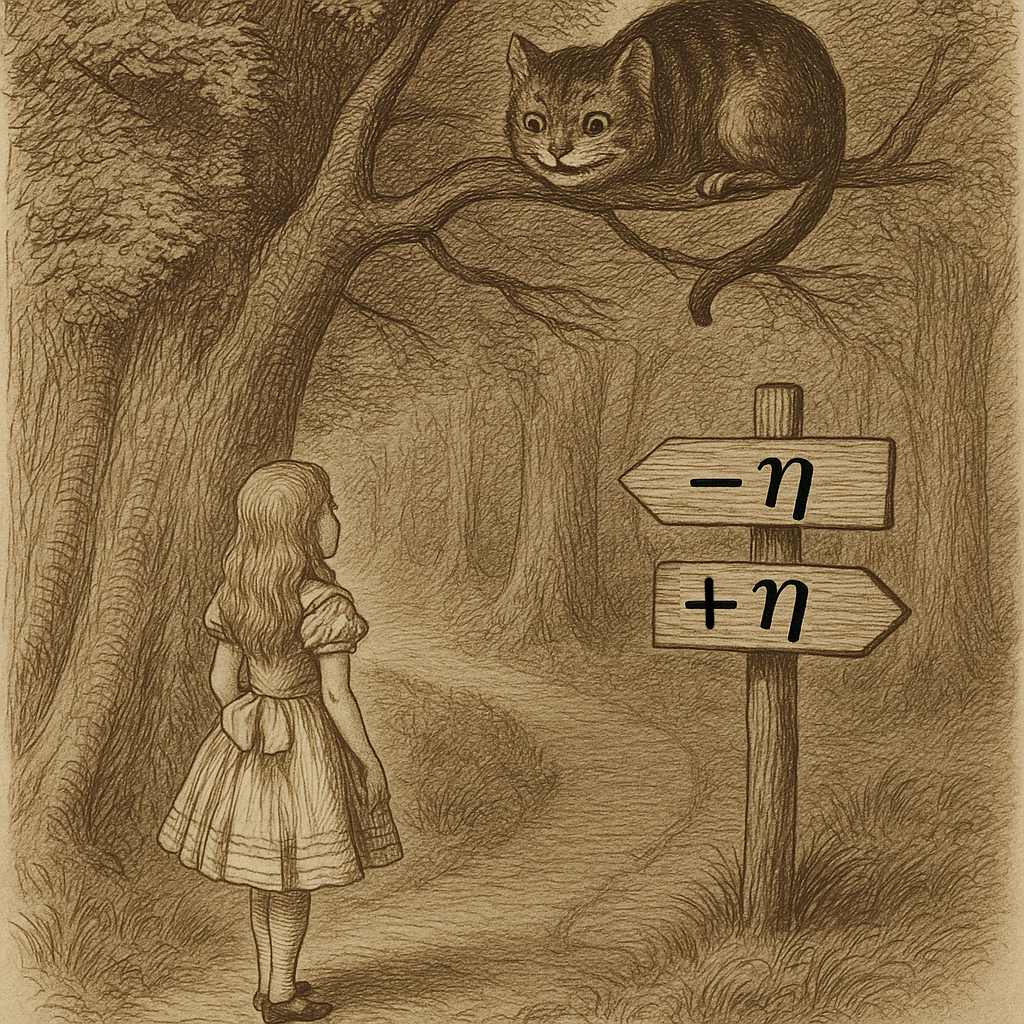
\includegraphics[height=0.5\textheight]{learning_rule}
	\caption{$w = w + \eta(y -  \hat{y})$}
	\label{fig:learningrule}
\end{figure}
	
\end{frame}


\begin{frame}{From Rosenblatt's Rule to Gradient Descent (2)}

	\textbf{Why Gradient Descent?}
	\begin{itemize}
		\item Defines an explicit \emph{loss function} $L(\bm{w})$ (e.g., squared error, cross-entropy).
		\item Updates are derived systematically:
		\[
		\bm{w}_{t+1} = \bm{w}_t - \eta \,\nabla L(\bm{w}_t).
		\]
		\item Extends naturally to multi-layer networks and differentiable activations.
		\item Provides convergence guarantees (under assumptions) and flexibility with optimizers.
	\end{itemize}
	
	\textbf{Key insight:} Gradient descent generalizes Rosenblatt’s idea, moving from “correction by mistake” to “optimization by minimizing a loss.”
\end{frame}



\section{Gradient}

\frame{ 
	\frametitle{Gradient}
	\begin{itemize}
		\item If $f$ is a function of two variables $x$ and $y$, then the gradient of $f$ is the vector function $\nabla f$ defined by 
		
		\begin{equation}
		\nabla f(x,y) = \left[ f_x(x,y), f_y(x,y) \right] = \frac{\partial f}{ \partial x} i + \frac{\partial f}{ \partial y} j 	
		\end{equation}
	\end{itemize}
	\begin{flushright}
		[Stewart, Multivariate Calculus]
	\end{flushright}
}


\frame{
	\frametitle{Gradient}
	\begin{itemize}
	\item It is a vector valued function. 
	$$y = f(w_1,w_2, \times, w_n)$$
	$$\nabla f = \left[ \begin{array}{c}
	\frac{\partial f}{ \partial w_1} \\ 
	\frac{\partial f}{ \partial w_2} \\
	\dots \\
	\frac{\partial f}{ \partial w_n}
	\end{array}  \right] $$
	\end{itemize}
\begin{center}
	\includegraphics[height=0.4\textheight]{../../../../../Downloads/Gemini_Generated_Image_ym00p0ym00p0ym00}
\end{center}
}


\begin{frame}
	\frametitle{Gradient}
	\begin{itemize}
			\item Example	
		$$f(x,y) = \left[ \begin{array}{c}  xy \\ xy \end{array}  \right] $$
		$$\nabla f = ?$$
		\pause
		$$\nabla f = \left[ \begin{array}{c}
			y\\ 
			x
		\end{array}  \right] $$
			\item A nice explanation: khanacademy.org/.../gradient
	\end{itemize}
\end{frame}


\begin{frame}{Summary: Fundamental Differentiation Rules}
	\small
	\begin{columns}[t]
		\begin{column}{0.48\textwidth}
			\begin{block}{Basic Rules}
				\begin{itemize}
					\item \textbf{Constant:} $\frac{d}{dx}(c) = 0$
					\item \textbf{Power:} $\frac{d}{dx}(x^n) = nx^{n-1}$
					\item \textbf{Constant Multiple:} $\frac{d}{dx}[cf(x)] = c f'(x)$
					\item \textbf{Sum/Difference:} $(f \pm g)' = f' \pm g'$
				\end{itemize}
			\end{block}
		\end{column}
		
		\begin{column}{0.48\textwidth}
			\begin{block}{Operations \& Composition}
				\begin{itemize}
					\item \textbf{Product Rule:} 
					\[ (fg)' = f'g + fg' \]
					\item \textbf{Quotient Rule:} 
					\[ \left(\frac{f}{g}\right)' = \frac{f'g - fg'}{g^2} \]
					\item \textbf{Chain Rule:} 
					\[ [f(g(x))]' = f'(g(x)) \cdot g'(x) \]
				\end{itemize}
			\end{block}
		\end{column}
	\end{columns}
	
	%\vspace{0.3cm}
	%\begin{exampleblock}{Quick Example (Chain Rule)}
	%	Let $y = (x^2 + 1)^3 \implies y' = 3(x^2 + 1)^2 \cdot (2x) = 6x(x^2 + 1)^2$
	%\end{exampleblock}
\end{frame}


\section{Gradient descent}

\begin{frame}
\frametitle{Gradient descent}
\begin{itemize}
	\item Goal. Minimize a differentiable objective
	\[
	\min_{\bm{\theta}\in\mathbb{R}^d} f(\bm{\theta}), \qquad \nabla f(\bm{\theta}) \text{ available.}
	\]
	\item Descent direction. The gradient points to steepest \emph{increase}. Move in the opposite direction:
	\[
	\bm{\theta}_{t+1} \;=\; \bm{\theta}_t \;-\; \eta \,\nabla f(\bm{\theta}_t),
	\]
	where $\eta>0$ is the \emph{learning rate / step size}.
\end{itemize}
\end{frame}

	
	% -------------------- Slide 1 --------------------
	\begin{frame}{Idea}

		\textbf{Geometric intuition.}
		$$y = \theta^2$$
		\begin{center}
			\begin{tikzpicture}[scale=0.9]
				% axes
				\draw[->] (-3.5,0) -- (3.8,0) node[below] {$\theta$};
				\draw[->] (0,-0.2) -- (0,5) node[left] {$f(\theta)$};
				% parabola
				\draw[thick, domain=-3.2:3.2, samples=100] plot (\x,{0.35*(\x)^2+0.6});
				% steps
				\foreach \x/\lab in {2.8/$\theta_0$,1.6/$\theta_1$,0.9/$\theta_2$,0.5/$\theta_3$} {
					\fill (\x,{0.35*(\x)^2+0.6}) circle (1.6pt);
					\node[above right] at (\x,{0.35*(\x)^2+0.6}) {\small \lab};
				}
				\draw[->,>=stealth] (2.8,3.34) -- (1.6,1.50);
				\draw[->,>=stealth] (1.6,1.50) -- (0.9,0.89);
				\draw[->,>=stealth] (0.9,0.89) -- (0.5,0.69);
				\node[below right] at (0.05,0.6) {\small $\theta^\star$};
				\fill (0,0.6) circle (1.6pt);
			\end{tikzpicture}
		\end{center}
		
	\end{frame}
	
	% -------------------- Slide 2 --------------------
	\begin{frame}{Algorithm \& Variants}
		\textbf{Basic algorithm}
		\begin{enumerate}
			\item Choose initial point $\bm{\theta}_0$ and step size $\eta \in (0,1)$.
			\item For $t=0,1,2,\dots$ until convergence:
			\begin{enumerate}
				\item Compute gradient $\bm{g}_t=\nabla f(\bm{\theta}_t)$.
				\item Update $\bm{\theta}_{t+1}=\bm{\theta}_t-\eta\,\bm{g}_t$.
			\end{enumerate}
		\end{enumerate}
		
		\vspace{0.3em}
		\textbf{Choosing the step size}
		\begin{itemize}
			\item Fixed $\eta$: simple; may under/overshoot.
			\item Schedules: $\eta_t=\eta_0/(1+\alpha t)$ or cosine decay, etc.
			\item Line search: adapt $\eta_t$ each step to satisfy sufficient decrease.
		\end{itemize}
	\end{frame}
	
	% -------------------- Slide 3 --------------------
	\begin{frame}{Convergence \& Practical Tips}
		\textbf{Theory snapshots}
		\begin{itemize}
			\item If $f$ is $L$-smooth and $\mu$-strongly convex, GD with $0<\eta<2/L$ converges linearly to $\bm{\theta}^\star$:
			\[
			\|\bm{\theta}_{t}-\bm{\theta}^\star\| \le (1-\mu\eta)^t \|\bm{\theta}_0-\bm{\theta}^\star\|.
			\]
			\item For general non-convex $f$, GD decreases $f$ and often converges to a \emph{stationary point} where $\|\nabla f\|$ is small.
		\end{itemize}
		
		%\textbf{Practical tips}
		%\begin{itemize}
		%	\item \textit{Scale features / normalize inputs} to reduce pathological curvature.
		%	\item Monitor $f(\bm{\theta}_t)$ and $\|\nabla f(\bm{\theta}_t)\|$.
		%	\item Check for too-large $\eta$ (divergence/oscillation) or too-small $\eta$ (slow progress).
		%\end{itemize}
	\end{frame}


\frame{
\frametitle{References}
 \begin{itemize}
 	\item Goodfellow, Ian, et al. Deep learning. Vol. 1. No. 2. Cambridge: MIT press, 2016.
 	\item Stewart, James, Daniel K. Clegg, and Saleem Watson. Calculus: early transcendentals. Cengage Learning, 2020.
    \item Khan Academy, Calculus.
 \end{itemize}
}


\end{document}